
\documentclass[journal,12pt,twocolumn]{IEEEtran}
%
\usepackage{setspace}
\usepackage{gensymb}
\usepackage{xcolor}
\usepackage{caption}
\usepackage{circuitikz}
%\usepackage{subcaption}
%\doublespacing
\singlespacing
\usepackage{float}
%\usepackage{graphicx}
%\usepackage{amssymb}
%\usepackage{relsize}
\usepackage[cmex10]{amsmath}
\usepackage{mathtools}
%\usepackage{amsthm}
%\interdisplaylinepenalty=2500
%\savesymbol{iint}
%\usepackage{txfonts}
%\restoresymbol{TXF}{iint}
%\usepackage{wasysym}
\usepackage{hyperref}
\usepackage{amsthm}
\usepackage{mathrsfs}
\usepackage{txfonts}
\usepackage{stfloats}
\usepackage{cite}
\usepackage{cases}
\usepackage{subfig}
%\usepackage{xtab}
\usepackage{longtable}
\usepackage{multirow}
%\usepackage{algorithm}
%\usepackage{algpseudocode}
%\usepackage{enumerate}
\usepackage{enumitem}
\usepackage{mathtools}
%\usepackage{iithtlc}
%\usepackage[framemethod=tikz]{mdframed}
\usepackage{listings}
\let\vec\mathbf


%\usepackage{stmaryrd}


%\usepackage{wasysym}
%\newcounter{MYtempeqncnt}
\DeclareMathOperator*{\Res}{Res}
%\renewcommand{\baselinestretch}{2}
\renewcommand\thesection{\arabic{section}}
\renewcommand\thesubsection{\thesection.\arabic{subsection}}
\renewcommand\thesubsubsection{\thesubsection.\arabic{subsubsection}}

\renewcommand\thesectiondis{\arabic{section}}
\renewcommand\thesubsectiondis{\thesectiondis.\arabic{subsection}}
\renewcommand\thesubsubsectiondis{\thesubsectiondis.\arabic{subsubsection}}

%\renewcommand{\labelenumi}{\textbf{\theenumi}}
%\renewcommand{\theenumi}{P.\arabic{enumi}}

% correct bad hyphenation here
\hyphenation{op-tical net-works semi-conduc-tor}

\lstset{
language=Python,
frame=single, 
breaklines=true,
columns=fullflexible
}



\begin{document}
%

\theoremstyle{definition}
\newtheorem{theorem}{Theorem}[section]
\newtheorem{problem}{Problem}
\newtheorem{proposition}{Proposition}[section]
\newtheorem{lemma}{Lemma}[section]
\newtheorem{corollary}[theorem]{Corollary}
\newtheorem{example}{Example}[section]
\newtheorem{definition}{Definition}[section]
%\newtheorem{algorithm}{Algorithm}[section]
%\newtheorem{cor}{Corollary}
\newcommand{\BEQA}{\begin{eqnarray}}
\newcommand{\EEQA}{\end{eqnarray}}
\newcommand{\define}{\stackrel{\triangle}{=}}
\newcommand{\myvec}[1]{\ensuremath{\begin{pmatrix}#1\end{pmatrix}}}
\newcommand{\mydet}[1]{\ensuremath{\begin{vmatrix}#1\end{vmatrix}}}
\newcommand{\rect}{\mathop{\mathrm{rect}}}
\newcommand{\sinc}{\mathop{\mathrm{sinc}}}
\bibliographystyle{IEEEtran}
%\bibliographystyle{ieeetr}
\providecommand{\system}[1]{\overset{\mathcal{#1}}{ \longleftrightarrow}}
\providecommand{\nCr}[2]{\,^{#1}C_{#2}} % nCr
\providecommand{\nPr}[2]{\,^{#1}P_{#2}} % nPr
\providecommand{\mbf}{\mathbf}
\providecommand{\pr}[1]{\ensuremath{\Pr\left(#1\right)}}
\providecommand{\qfunc}[1]{\ensuremath{Q\left(#1\right)}}
\providecommand{\sbrak}[1]{\ensuremath{{}\left[#1\right]}}
\providecommand{\lsbrak}[1]{\ensuremath{{}\left[#1\right.}}
\providecommand{\rsbrak}[1]{\ensuremath{{}\left.#1\right]}}
\providecommand{\brak}[1]{\ensuremath{\left(#1\right)}}
\providecommand{\lbrak}[1]{\ensuremath{\left(#1\right.}}
\providecommand{\rbrak}[1]{\ensuremath{\left.#1\right)}}
\providecommand{\cbrak}[1]{\ensuremath{\left\{#1\right\}}}
\providecommand{\lcbrak}[1]{\ensuremath{\left\{#1\right.}}
\providecommand{\rcbrak}[1]{\ensuremath{\left.#1\right\}}}
\theoremstyle{remark}
\newtheorem{rem}{Remark}
\newcommand{\sgn}{\mathop{\mathrm{sgn}}}
\providecommand{\abs}[1]{\left\vert#1\right\vert}
\providecommand{\res}[1]{\Res\displaylimits_{#1}} 
\providecommand{\norm}[1]{\lVert#1\rVert}
\providecommand{\mtx}[1]{\mathbf{#1}}
\providecommand{\mean}[1]{E\left[ #1 \right]}
\providecommand{\fourier}{\overset{\mathcal{F}}{ \rightleftharpoons}}
\providecommand{\ztrans}{\overset{\mathcal{Z}}{ \rightleftharpoons}}

%\providecommand{\hilbert}{\overset{\mathcal{H}}{ \rightleftharpoons}}
\providecommand{\system}{\overset{\mathcal{H}}{ \longleftrightarrow}}
	%\newcommand{\solution}[2]{\textbf{Solution:}{#1}}
\newcommand{\solution}{\noindent \textbf{Solution: }}
\providecommand{\dec}[2]{\ensuremath{\overset{#1}{\underset{#2}{\gtrless}}}}
\numberwithin{equation}{section}
%\numberwithin{equation}{subsection}
%\numberwithin{problem}{subsection}
%\numberwithin{definition}{subsection}
\makeatletter
\@addtoreset{figure}{problem}
\makeatother

\let\StandardTheFigure\thefigure
%\renewcommand{\thefigure}{\theproblem.\arabic{figure}}
\renewcommand{\thefigure}{\theproblem}


%\numberwithin{figure}{subsection}

\def\putbox#1#2#3{\makebox[0in][l]{\makebox[#1][l]{}\raisebox{\baselineskip}[0in][0in]{\raisebox{#2}[0in][0in]{#3}}}}
     \def\rightbox#1{\makebox[0in][r]{#1}}
     \def\centbox#1{\makebox[0in]{#1}}
     \def\topbox#1{\raisebox{-\baselineskip}[0in][0in]{#1}}
     \def\midbox#1{\raisebox{-0.5\baselineskip}[0in][0in]{#1}}

\vspace{3cm}

\title{ 
%\logo{
%}
Fourier 
%	\logo{Octave for Math Computing }
}
%\title{
%	\logo{Matrix Analysis through Octave}{\begin{center}\includegraphics[scale=.24]{tlc}\end{center}}{}{HAMDSP}
%}



\author{ Mannem Charan AI21BTECH11019 %<-this  stops a space
}
\maketitle


\tableofcontents


\renewcommand{\thefigure}{\theenumi}
\renewcommand{\thetable}{\theenumi}



\bigskip

\begin{abstract}
This manual provides a simple introduction to Fourier Series
\end{abstract}
\section{Periodic Function}
Let
\begin{align}
	x(t) &= A_0\abs{\sin\brak{2\pi f_0 t}}
	\label{eq:10-orig-diff-def}
\end{align}
\begin{enumerate}[label=\thesection.\arabic*
,ref=\thesection.\theenumi]
\item Plot $x(t)$. \\
 \solution Download the python code for the plot of $x(t)$,
  \begin{lstlisting}
wget https://github.com/Charanyash/EE3900-Digital_Signal_Processing/blob/master/Fourier/Codes/1.1.py
   \end{lstlisting}
Then run the following command,
 \begin{lstlisting}
python3 1.1.py
\end{lstlisting}
 \begin{figure}
	 \centering
	 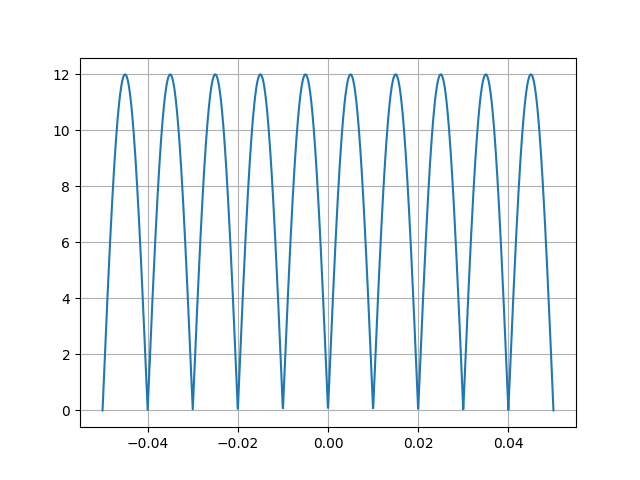
\includegraphics[width = \columnwidth]{Figs/1.1.png}
	 \caption{}
	 \label{fig:1}
 \end{figure}
\item Show that $x(t)$ is periodic and find its period. \\
 \solution We will say a function $f(x)$ is periodic if there exists a real number $T$, such that
  \begin{align}
	  f(x + T) &= f(x)
  \end{align}
  So for the given $x(t)$ which is absolute sinusoidal function is also periodic which can be seen in the fig $\ref{fig:1}$.For the period, consider the following 
   \begin{align}
	   x(t + \frac{1}{2f_0}) &= \abs{\sin\brak{2\pi f_0 \brak{t + \frac{1}{2f_0}}}} \\
	                         &= \abs{\sin\brak{2\pi f_0t + \pi}} \\
				 &= \abs{-\sin\brak{2\pi f_0 t}} \\
				 &= \abs{\sin\brak{2\pi f_0 t}}
   \end{align}
This shows that the $x(t)$ is periodic with period $\frac{1}{2f_0}$.
\end{enumerate}
\section{Fourier Series}
Consider $A_0 =12$ and $f_0 = 50$ for all numerical calculations.
\begin{enumerate}[label=\thesection.\arabic*,ref=\thesection.\theenumi]
\item If
%\cite{proakis_dsp}
\begin{align}
	x(t) = \sum_{k = -\infty}^{\infty}c_ke^{j2\pi kf_0 t}
\label{eq:one-Z-complex}
\end{align}
show that 
\begin{align}
	c_k = f_0\int_{-\frac{1}{2f_0}}^{\frac{1}{2f_0}}x(t)e^{-j2\pi kf_0 t}\, dt
\label{eq:one-Z}
\end{align}
\solution 
To show that, 
\begin{align}
	c_k = f_0\int_{-\frac{1}{2f_0}}^{\frac{1}{2f_0}}x(t)e^{-j2\pi kf_0 t}\, dt
\end{align}
Consider the RHS and use $\eqref{eq:one-Z-complex}$,
  \begin{align}
	  f_0\int_{-\frac{1}{2f_0}}^{\frac{1}{2f_0}}x(t)e^{-j2\pi kf_0 t}\, dt &= f_0\int_{-\frac{1}{2f_0}}^{\frac{1}{2f_0}}\brak{\sum_{n = -\infty}^{\infty}c_ne^{j2\pi nf_0 t}}
e^{-j2\pi kf_0 t}\\
			     &= f_0\sum_{n = -\infty}^{\infty}\int_{-\frac{1}{2f_0}}^{\frac{1}{2f_0}}c_ne^{j 2\pi\brak{n-k}f_0t} \,dt 
  \end{align}
  And the definite integral evaluates to, 
   \begin{align}
	   \int{-\frac{1}{2f_0}}^{\frac{1}{2f_0}}e^{j 2\pi \brak{n-k}f_0t} = \begin{cases}
		                                                                 \frac{1}{f_0} , & n = k \\
										  0            , & n \neq k
									      \end{cases}
   \end{align}
Using that, 
     \begin{align}
	     f_0\int_{-\frac{1}{2f_0}}^{\frac{1}{2f_0}}x(t)e^{-j2\pi kf_0 t}\, dt &= f_0\brak{\frac{c_k}{f_0}} \\
	                                                                           &= c_k
     \end{align}
Hence proved.

	\item Find $c_k$ for 
	$\eqref{eq:10-orig-diff-def}$ \\
	\solution To find $c_k$ for given $x(t)$ we will use $\eqref{eq:one-Z}$,
	  \begin{align}
		  c_k &= f_0\int_{-\frac{1}{2f_0}}^{\frac{1}{2f_0}}x(t)e^{-j2\pi kf_0 t}\, dt \\
		      &= A_0f_0\int_{0}^{\frac{1}{2f_0}}\sin\brak{2\pi f_0t}\brak{e^{-j2\pi kf_0t} + e^{-j2\pi kf_0t}} \\
		      & \brak{\because \int_{-a}^{a} f(x)dx = \int_{0}^{a}f(a) + f(-a)\,dx}\nonumber \\
		      &= A_0f_0\int_{0}^{\frac{1}{2f_0}}\sin\brak{2\pi f_0 t}\brak{2\cos\brak{2\pi k f_0t}} \\
		      &= A_0f_0\int_{0}^{\frac{1}{2f_0}}\brak{\sin\brak{2\pi f_0t\brak{1-k}} + \sin\brak{2\pi f_0t\brak{1 + k}}} \\
		      &= A_0f_0\sbrak{\frac{\cos\brak{2\pi f_0t\brak{k -1}}}{2 \pi f_0\brak{k-1}} - \frac{\cos\brak{2\pi f_0t\brak{k+1}}}{2 \pi f_0\brak{k+1}}}_{0}^{\frac{1}{2f_0}}\\
		      &= A_0\frac{\brak{\cos\brak{\pi \brak{k-1}} - 1}}{2\pi \brak{k-1}} - \frac{\brak{\cos\brak{\pi \brak{k+1}} -1}}{2\pi \brak{k+1}}\\
		      &= \frac{A_0\brak{(-1)^{k+1} -1}}{2\pi}\sbrak{\frac{1}{k-1} - \frac{1}{k+1}} \\
		      &= \frac{A_0\brak{(-1)^{k+1} - 1}}{\pi\brak{k^{2} -1}}
	  \end{align}

  In other words,
     \begin{align}
	     c_k = \begin{cases}
		         0 &, \text{k is odd} \\
			 \frac{2A_0}{\pi\brak{1 - k^2}} &, \text{ k is even}
		 \end{cases}\label{eq:c_k}
     \end{align}
\item Verify 
	$\eqref{eq:10-orig-diff-def}$
	using python.\\
\solution Download the python code from the below link
   \begin{lstlisting}
wget  https://github.com/Charanyash/EE3900-Digital_Signal_Processing/blob/master/Fourier/Codes/2.3.py
\end{lstlisting}
Then run the following command in terminal
 \begin{lstlisting}
python3 2.3.py
\end{lstlisting}

\begin{figure}[!ht]
 \centering
 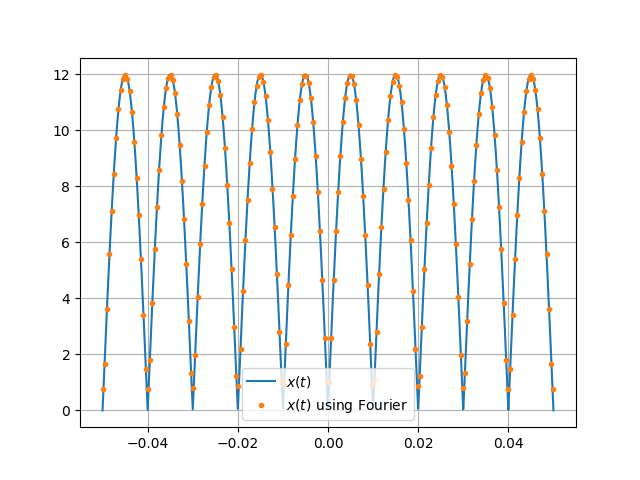
\includegraphics[width = \columnwidth]{Figs/2.3.png}
 \caption{}
 \label{fig:fourier}
\end{figure}

\item Show that 
\begin{align}
	x(t) = \sum_{k = 0}^{\infty}\brak{a_k\cos{j2\pi kf_0 t}+b_k\sin{\j2\pi kf_0 t}}
\label{eq:one-Z-real}
\end{align}
and obtain the formulae for $a_k$ and $b_k$.\\
\solution From $\eqref{eq:one-Z-complex}$,
 \begin{align}
	 x(t) &= \sum_{k = -\infty}^{\infty}c_ke^{-j 2\pi kf_0t} \\
	      &= \sum_{k= -\infty}^{\infty}c_k\brak{\cos\brak{2 \pi kf_0t} - \j \sin\brak{2 \pi kf_0t}} \\
	      &= c_0 + \sum_{k = 1}^{\infty}\cos\brak{2 \pi kf_0t}\brak{c_k + c_{-k}} \nonumber \\
	       & + \sum_{k=1}^{\infty}\brak{c_k - c_{-k}}\sin\brak{2 \pi kf_0t}
 \end{align}
  Now by comparing we can write $a_k$ and $b_k$ as ,
   \begin{align}
      a_k = \begin{cases}
	       c_0 &, k = 0\\
	       c_k + c_{-k} &, k \neq 0 
	    \end{cases}
   \end{align}
   \begin{align}
	b_k = c_k - c_{-k}
   \end{align}
\item Find $a_k$ and $b_k$ for 
	$\eqref{eq:10-orig-diff-def}$\\
 \solution Using $\eqref{eq:c_k}$, we will get $a_k$ and $b_k$ as,
    \begin{align}
       a_k = \begin{cases}
	       0 &, \text{k is odd}\\
	       \frac{2A_0}{\pi} &, k = 0 \\
	       \frac{4A_0}{\pi\brak{1 - k^{2}}} &, \text{k is even} \,-\cbrak{0}
	     \end{cases}
     \end{align}
    \begin{align}
	    b_k = 0 \forall k
    \end{align}
    Note that $c_k = c_{-k} \forall k$.
\item Verify 
$\eqref{eq:one-Z-real}$
using python.\\
\solution Download the python code from the below link,
\begin{lstlisting}
 wget https://github.com/Charanyash/EE3900-Digital_Signal_Processing/blob/master/Fourier/Codes/2.6.py
\end{lstlisting}
Then run the following command,
 \begin{lstlisting}
python3 2.6.py
 \end{lstlisting}

 \begin{figure}[!ht]
  \centering
  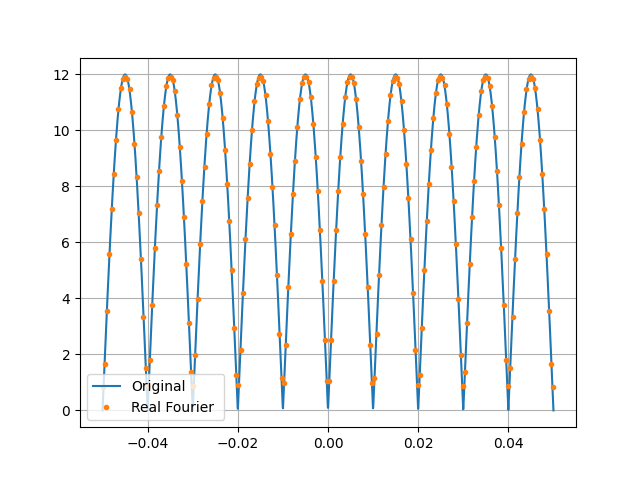
\includegraphics[width = \columnwidth]{Figs/2.6.png}
  \caption{}
  \label{fig:real-fou}
\end{figure}

\end{enumerate}
\section{Fourier Transform}

 

\begin{enumerate}[label=\thesection.\arabic*
,ref=\thesection.\theenumi]
\item 
	\begin{align}
		\delta(t)&=0, \quad t\neq0
\\
		\int_{-\infty}^{\infty}\delta(t) \, dt&= 1
	\end{align}
 \item The Fourier Transform of $g(t)$ is
 \begin{align}
	 G(f)=\int_{-\infty}^{\infty}g(t)e^{-j2\pi ft}\,dt\label{def:fourier}
 \end{align}
 \item Show that 
 \begin{align}
	 g(t-t_0)&\system{F}G(f)e^{-j2\pi ft_0}\\
 \end{align}
 \solution Using the definition $\eqref{def:fourier}$,
   \begin{align}
	   \mathcal{F}\cbrak{g(t-t_0)} &= \int_{-\infty}^{\infty}g(t-t_0)e^{-j2\pi ft}\,dt \\
	                               &= \int_{-\infty}^{\infty}g(k)e^{-j2\pi f\brak{t_0 + k}} \, dk \\
				       &= e^{-j2\pi ft_0} \int_{-\infty}^{\infty}g(k)e^{-j2\pi fk} \, dk \\
				       &= G(f)e^{-j2\pi ft_0}
   \end{align}
   Hence proved.
 \item Show that 
 \begin{align}
	 G(t)&\system{F}g(-f)
 \end{align}
  \solution We know that ,
    \begin{align}
	g(t) &\system{F}G(f)
    \end{align}
    So we can write,
     \begin{align}
	g(t) &= \int_{-\infty}^{\infty}G(f)e^{j 2\pi ft} \, df \\
	     &= \int_{-\infty}^{\infty}G(k) e^{j 2 \pi kt} \, dk \\
	\implies g(-f) &= \int_{-\infty}^{\infty} G(k) e^{-j 2 \pi kf} \, dk \\
	               &= \mathcal{F}\cbrak{G(t)}
     \end{align}
     Hence proved.
 \item $\delta(t)\system{F}?$ \\
   \solution We know that,
     \begin{align}
	 \int \delta(t-t_0)f(t) &= f(t_0)
      \end{align}
    So, 
     \begin{align}
	\delta(t)\system{F} &= \int_{-\infty}^{\infty}\delta(t)e^{-j 2 \pi ft}dt \\
	                    &= e^{-\j 2 \pi ft}\vert_{t = 0} \\
			    &= 1
     \end{align}
 \item $e^{-j2\pi f_0t}\system{F}?$\\
  \solution From above we know that,
    \begin{align}
	    \delta(t) &\system{F} 1 \\
            \delta(t-t_0) &\system{F} 1.e^{-j 2 \pi ft_0}\\
	    \implies e^{-j 2 \pi tf_0} &\system{F} \delta(-f-f_0) \\
	    \implies e^{- j 2\pi tf_0} & \system{F} \delta(f + f_0)
    \end{align}
 \item $\cos(2\pi f_0t)\system{F}?$\\
  \solution We know that,
   \begin{align}
	   \cos(2 \pi f_0t) &= \frac{e^{j 2 \pi f_0t} + e^{ -j 2 \pi f_0t}}{2}
   \end{align}
   Now if we apply fourier transform on both sides,
    \begin{align}
	    \mathcal{F}\cbrak{\cos 2 \pi f_0t} &= \frac{1}{2} \sbrak{ \delta\brak{f - f_0} + \delta\brak{f + f_0}}
    \end{align}

    $\therefore \cos(2 \pi f_0t) \system{F} \frac{ \delta\brak{f - f_0} + \delta\brak{f + f_0}}{2}$
 \item Find the Fourier Transform of $x(t)$ and plot it.  Verify using python.\\
  \solution To find the fourier transform of $x(t)$ we can use the fourier series expansion,
    \begin{align}
	    x(t) &= \sum_{k = -\infty}^{\infty}c_ke^{j 2 \pi kf_0t} \\
	    \implies \mathcal{F}\cbrak{x(t)} &= \sum_{k = -\infty}^{\infty}c_k \mathcal{F}\cbrak{e^{j 2 \pi kf_0t}}\\
					 &= \sum_{k = -\infty}^{\infty}c_k \delta\brak{f - kf_0}
    \end{align}

    Now using $\eqref{eq:c_k}$, 
      \begin{align}
	      \mathcal{F}\cbrak{x(t)} &= \sum_{ k \, \text{is even}}\frac{2A_0\delta\brak{f-kf_0}}{\pi\brak{1 - k^2}} 
      \end{align}

      The same can be seen in Fig $\ref{fig:four_trans-x}$. Download the python code from the below link,
 \begin{lstlisting}
 wget  https://github.com/Charanyash/EE3900-Digital_Signal_Processing/blob/master/Fourier/Codes/3.8.py
\end{lstlisting}
Then run the following command in terminal,
 \begin{lstlisting}
python3 3.8.py
  \end{lstlisting}
  \begin{figure}[!ht]
   \centering
   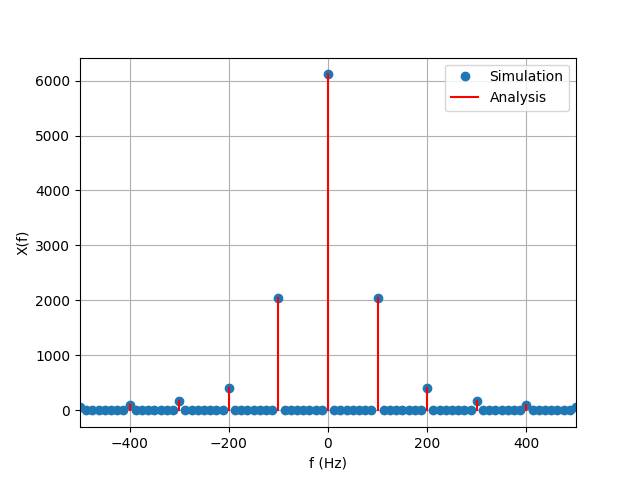
\includegraphics[width = \columnwidth]{Figs/3.8.png}
   \caption{}
   \label{fig:four_trans-x}
  \end{figure}
 \item Show that 
 \begin{align}
	 \rect{t} \system{F} \sinc{f}
 \end{align}
 Verify using python.\\
 \solution The $rect(t)$ is defined as,
   \begin{align}
	   \rect{t} = \begin{cases}
		   1   &, \abs{t} \leq \frac{1}{2} \\
			 0   &, \text{otherwise}
		     \end{cases}
   \end{align}

   So fourier transform will be,
    \begin{align}
	    \mathcal{F}\cbrak{\rect{t}} &= \int_{-\infty}^{\infty}\rect{t}e^{-j 2 \pi ft}\,dt \\
				       &= \int_{-\frac{1}{2}}^{\frac{1}{2}} e^{ -j 2 \pi ft} \, dt\\
				       &= \int_{0}^{\frac{1}{2}} e^{-j 2 \pi ft} + e^{j 2 \pi ft} \, dt \\
				       &= 2\int_{0}^{\frac{1}{2}}\cos\brak{2 \pi ft} \,dt \\
				       &= 2 \sbrak{\frac{\sin\brak{2 \pi ft}}{2 \pi f}}_{0}^{\frac{1}{2}} \\
				       &= \frac{\sin\brak{\pi f}}{\pi f} \\
				       &= \sinc{f} 
   \end{align}

   Download the python code from the below link,
    \begin{lstlisting}
wget  https://github.com/Charanyash/EE3900-Digital_Signal_Processing/blob/master/Fourier/Codes/3.9.py
\end{lstlisting}
  Run the following command,
   \begin{lstlisting}
python3 3.9.py
\end{lstlisting}
 \begin{figure}[!ht]
  \centering
  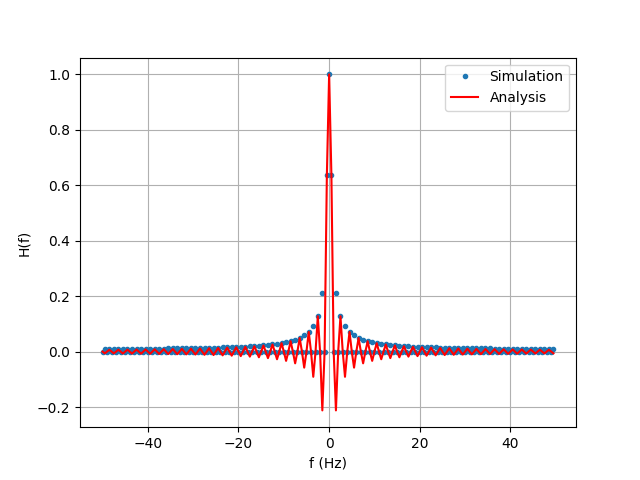
\includegraphics[width = \columnwidth]{Figs/3.9.png}
  \caption{}
  \label{fig:four_rect}
 \end{figure}
\item 
$	 \sinc{t}\system{F} ?$.  Verify using python.\\
 \solution From the duality property of Fourier Transform,
   \begin{align}
	   \rect{t} &\system{F} \sinc{f} \\
	   \implies \sinc{t} &\system{F} \rect{-f}
\end{align}
Since $\rect{t}$ is an even function,
  \begin{align}
  \sinc{t} \system{F} \rect{f}
  \end{align}

  Download the python code from the following link,
   \begin{lstlisting}
wget  https://github.com/Charanyash/EE3900-Digital_Signal_Processing/blob/master/Fourier/Codes/3.10.py
   \end{lstlisting}
   Then run the following command,
    \begin{lstlisting}
python3 3.10.py
    \end{lstlisting}

    \begin{figure}[!ht]
	\centering
	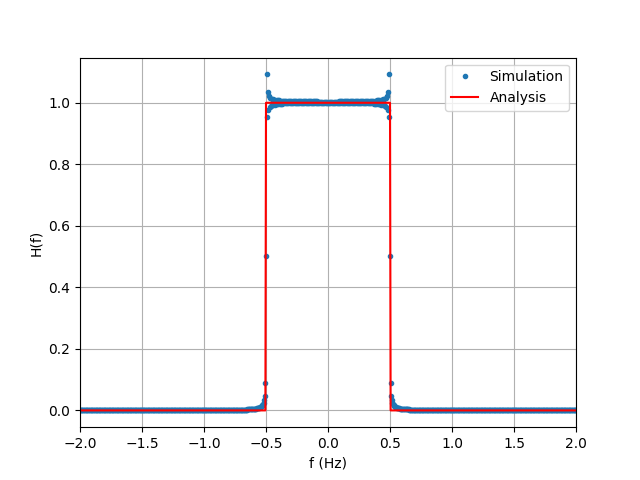
\includegraphics[width = \columnwidth]{Figs/3.10.png}
	\caption{}
	\label{fig:four_sinc}
    \end{figure}

\end{enumerate}
\section{Filter}\begin{enumerate}[label=\thesection.\arabic*
,ref=\thesection.\theenumi]
\item Find $H(f)$ which transforms $x(t)$ to DC 5V. \\
	\solution Since we need a DC output of $5V$, we need a filter which will remove the higher frequencies i.e., a low-pass filter so that we can retrieve the zero frequency components. So we need a filter which only allows certain frequencies lower than a cuttoff frequency $\brak{f_c}$. \\
	One can use $rect(f)$ as a low-pass filter,
	 \begin{align}
		 H(f) = krect\brak{\frac{f}{2f_c}} = \begin{cases}
			                                 k  &, f \leq f_c \\
							 0  &, \text{otherwise}
						     \end{cases}
	 \end{align}
	 And $k$ is amplification factor which makes $a_0$ of $x(t)$ as $5V$. We can evaluate the same as,
	  \begin{align}
		  H\brak{0} &= \frac{Y\brak{0}}{X\brak{0}} \\
		    k    &= \frac{5}{\frac{2A_0}{\pi}} 
	  \end{align}
	  This makes the transfer function $H(f)$ as,
	   \begin{align}
		   H(f) &= \frac{5\pi}{2A_0}rect\brak{\frac{f}{2f_c}}
	   \end{align}
\item Find $h(t)$.\\
 \solution We know that,
  \begin{align}
	  sinc(t) &\system{F} rect(f) \\
	  sinc(2f_ct) &\system{F} \frac{1}{2f_c}rect(\frac{f}{2f_c})\\
	  \therefore \frac{10f_c\pi}{2A_0}sinc(2f_ct) &\system{F} \frac{5\pi}{2A_0}rect\brak{\frac{f}{2f_c}}
  \end{align}
  The impulse response will be,
   \begin{align}
	   h(t) &= \frac{5f_c \pi}{A_0}sinc(2f_ct)
   \end{align}
\item Verify your result using  through convolution. \\
 \solution Download the python code from the following link,
  \begin{lstlisting}
wget  https://github.com/Charanyash/EE3900-Digital_Signal_Processing/blob/master/Fourier/Codes/4.3.py
\end{lstlisting}
Then run the following command,
 \begin{lstlisting}
python3 4.3.py
  \end{lstlisting}
  \begin{figure}[!ht]
	\centering
	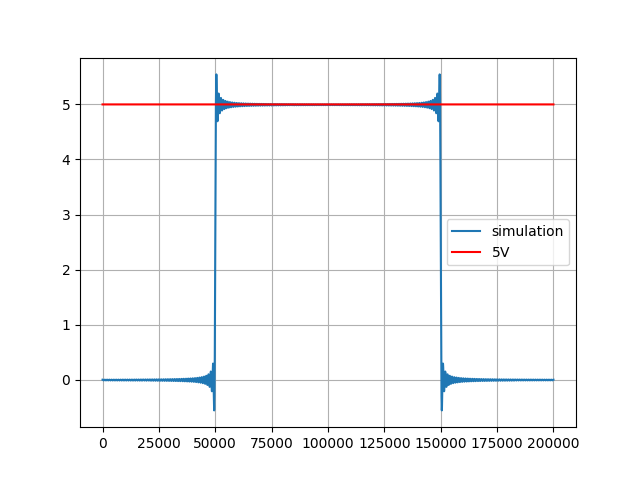
\includegraphics[width = \columnwidth]{Figs/4.3.png}
	\caption{}
	\label{fig:conv}
    \end{figure}

\end{enumerate}
\section{Filter Design}
\begin{enumerate}[label=\thesection.\arabic*
,ref=\thesection.\theenumi]
\item Design a Butterworth filter for $H(f)$.\\
	\solution The Butterworth filter has an amplitude response
	given by
	\begin{align}
		\abs{H\brak{f}}^2 = \frac{1}{\brak{1 + \brak{\frac{f}{f_c}}^{2n}}}
	\end{align}
	where $n$ is the order of the filter and $f_c$ is the cutoff
	frequency. The attenuation at frequency $f$ is given by 
	\begin{align}
		A &= -10\log_{10}\abs{H\brak{f}}^2 \\
		&= -20\log_{10}\abs{H\brak{f}}
		\label{eq:loss}
	\end{align}
	We consider the following design parameters for our
	lowpass analog Butterworth filter:
	\begin{enumerate}
		\item Passband edge, $f_p = 50$ Hz
		\item Stopband edge, $f_s = 100$ Hz
		\item Passband attenuation, $A_p = -1$ dB
		\item Stopband attenuation, $A_s = -20$ dB
	\end{enumerate}
	We are required to find a desriable order $n$ and cutoff
	frequency $f_c$ for the filter. From \eqref{eq:loss},
	\begin{align}
		A_p &= -10\log_{10}\sbrak{1 + \brak{\frac{f_p}{f_c}}^{2n}} \\
		A_s &= -10\log_{10}\sbrak{1 + \brak{\frac{f_s}{f_c}}^{2n}}
	\end{align}
	Thus,
	\begin{align}
		\brak{\frac{f_p}{f_c}}^{2n} = 10^{-\frac{A_p}{10}} - 1 \label{eq:fc1} \\
		\brak{\frac{f_s}{f_c}}^{2n} = 10^{-\frac{A_s}{10}} - 1 \label{eq:fc2}
	\end{align}
	Therefore, on dividing the above equations and solving for $n$,
	\begin{align}
		n = \frac{\log\brak{10^{-\frac{A_s}{10}} - 1} - 
			\log\brak{10^{-\frac{A_p}{10}} - 1}}{2\brak{\log{f_s} - \log{f_p}}}
	\end{align}
	In this case, making appropriate susbstitutions gives $n = 4.29$.
	Hence, we take $n = 5$. Solving for $f_c$ in $\eqref{eq:fc1}$ and
	\eqref{eq:fc2},
	\begin{align}
		f_{c1} = f_p\sbrak{10^{-\frac{A_p}{10}} - 1}^{-\frac{1}{2n}} = 57.23 \,Hz \\
		f_{c2} = f_s\sbrak{10^{-\frac{A_s}{10}} - 1}^{-\frac{1}{2n}} = 63.26 \,Hz
	\end{align}
	Hence, we take $f_c = \sqrt{f_{c1}f_{c2}} = 60 \, Hz$ approximately.
\item Design a Chebyschev filter for $H(f)$.\\
	\solution The Chebyshev filter has an amplitude response
	given by
	\begin{align}
		\abs{H\brak{f}}^2 = \frac{1}{\brak{1 + \epsilon^2C_n^2\brak{\frac{f}{f_c}}}}
	\end{align}
	where 
	\begin{enumerate}
		\item $n$ is the order of the filter
		\item $\epsilon$ is the ripple
		\item $f_c$ is the cutoff frequency 
		\item $C_n = \cosh^{-1}\brak{n\cosh{x}}$ denotes 
		the n\textsuperscript{th} order Chebyshev polynomial,
		given by
		\begin{align}
			c_n(x) =
			\begin{cases}
				\cos\brak{n\cos^{-1}x} & \abs{x} \le 1 \\
				\cosh\brak{n\cosh^{-1}x} & \textrm{otherwise}
			\end{cases}
			\label{eq:chebypol}
		\end{align}
	\end{enumerate}
	We are given the following specifications:
	\begin{enumerate}
		\item Passband edge (which is equal to 
		cutoff frequency), $f_p = f_c$
		\item Stopband edge, $f_s$
		\item Attenuation at stopband edge, $A_s$
		\item Peak-to-peak ripple $\delta$ in the passband.
		It is given in dB and is related to $\epsilon$ as
		\begin{align}
			\delta = 10\log_{10}\brak{1 + \epsilon^2}
			\label{eq:delta-eps}
		\end{align}
	\end{enumerate}
	and we must find a suitable $n$ and $\epsilon$. From
	\eqref{eq:delta-eps},
	\begin{align}
		\epsilon = \sqrt{10^{\frac{\delta}{10}} - 1}
		\label{eq:epsilon-del}
	\end{align}
	At $f_s > f_p = f_c$, using \eqref{eq:chebypol}, $A_s$ is given by
	\begin{align}
		A_s = -10\log_{10}\sbrak{1 + \epsilon^2c_n^2\brak{\frac{f_s}{f_p}}} \\
		\implies c_n\brak{\frac{f_s}{f_p}} = \frac{\sqrt{10^{-\frac{A_s}{10}} - 1}}{\epsilon} \\
		\implies n = \frac{\cosh^{-1}\brak{\frac{\sqrt{10^{-\frac{A_s}{10}} - 1}}{\epsilon}}}
		{\cosh^{-1}\brak{\frac{f_s}{f_p}}}
	\end{align}
	We consider the following specifications:
	\begin{enumerate}
		\item Passband edge/cutoff frequency, $f_p = f_c = 60 \, Hz$.
		\item Stopband edge, $f_s = 100 \,Hz $.
		\item Passband ripple, $\delta = 0.5 \,dB$
		\item Stopband attenuation, $A_s = -20 \,dB$
	\end{enumerate}
	$\epsilon = 0.35$ and $n = 3.68$. Hence, we take $n = 4$
	as the order of the Chebyshev filter.
\item Design a circuit for your Butterworth filter.\\
	\solution Looking at the table of normalized element values
	$L_k$, $C_k$, of the Butterworth filter for order 5, and noting
	that de-normalized values $L_k'$ and $C_k'$ are given by
	\begin{align}
		C_k' = \frac{C_k}{\omega_c} \qquad L_k' = \frac{L_k}{\omega_c}
	\end{align}
	De-normalizing these values, taking $f_c = 60$ Hz,
	\begin{align}
		C_1' = C_5' = 1.64 \mu F \\
		L_2' = L_4' = 4.29 \mu H \\
		C_3' = 5.31 \mu F
	\end{align}
	The L-C network is shown in Fig. \ref{fig:butter-filter}.
	\begin{figure}[!ht]
		\centering
		\begin{circuitikz} 
			\draw (0,0) to[short, o-o] (7,0);
			\draw (0,2) to [short, o-] (1,2) to [L, l=4.29 mH] (3.5,2) to [L, l=4.29 mH] (6,2) to[short, -o] (7,2);
			\draw (1,0) to[C, l=1.64 mF] (1,2);
			\draw (3.5,0) to[C, l=5.31 mF] (3.5,2);
			\draw (6,0) to[C, l=1.64 mF] (6,2);
		\end{circuitikz}
		\caption{L-C Butterworth Filter}
		\label{fig:butter-filter}
	\end{figure}
	
	\begin{figure}
		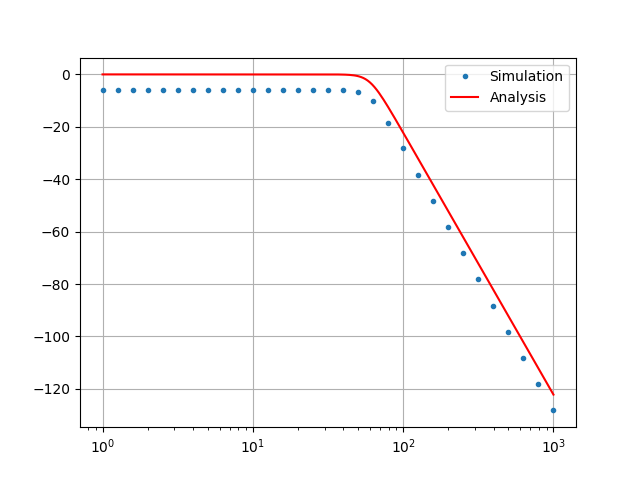
\includegraphics[width=\columnwidth]{Figs/5.3.png}
		\caption{Simulation of Butterworth filter.}
		\label{fig:sim-butter}
	\end{figure}
	Below python code plot the figure \ref{fig:sim-butter}
	\begin{lstlisting}
wget  https://github.com/Charanyash/EE3900-Digital_Signal_Processing/blob/master/Fourier/Codes/5.3.py
	\end{lstlisting}
\item Design a circuit for your Chebyschev filter.\\
	\solution Looking at the table of normalized element values
	of the Chebyshev filter for order 3 and 0.5 dB ripple,
	and de-nomrmalizing those values, taking $f_c = 50 \,Hz$,
	\begin{align}
		C_1' = 4.43 \mu F \\
		L_2' = 3.16 \mu F \\
		C_3' = 6.28 \mu F \\
		L_4' = 2.23 \mu F
	\end{align}
	The L-C network is shown in Fig. \ref{fig:cheby-filter}.
	\begin{figure}[!ht]
		\centering
		\begin{circuitikz} 
			\draw (0,0) to[short, o-o] (7,0); 
			\draw (1,0) to[C, l=4.43 mF] (1,2);
			\draw (3.5,0) to[C, l=6.28 mF] (3.5,2);
			\draw (0,2) to [short, o-] (1,2) to [L, l=3.16 mH] (3.5,2) to[L, l=2.23 mH] (6,2) to[short, -o] (7,2);
		\end{circuitikz}
		\caption{L-C Chebyshev Filter}
		\label{fig:cheby-filter}
	\end{figure}
	\begin{figure}
	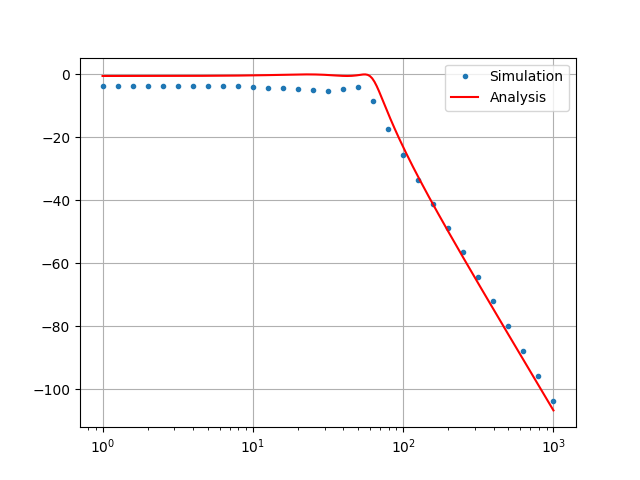
\includegraphics[width=\columnwidth]{Figs/5.4.png}
	\caption{Simulation of Chebyshev filter.}
	\label{fig:sim-cheby}
\end{figure}
	Below python code plot the figure \ref{fig:sim-cheby}
	\begin{lstlisting}
wget  https://github.com/Charanyash/EE3900-Digital_Signal_Processing/blob/master/Fourier/Codes/5.4.py
	\end{lstlisting}
\end{enumerate}


\end{document}
